\subsubsection{Neural Networks}
Another method that was researched by our group was the use of neural networks. This method, similar to Hidden Markov Models, uses graphs. Unlike the Hidden Markov Models though the connections between nodes of the graph represent how much one node affects the other; as opposed to conditional dependence. These connections are called weights. When multiple layers of these nodes and weights are connected they can be used to model very complex functions. These functions have been shown to be able to model various real life problems. Having become increasingly effective in the passed decade it was only natural that our research efforts led us in this direction.\par

\begin{center}
	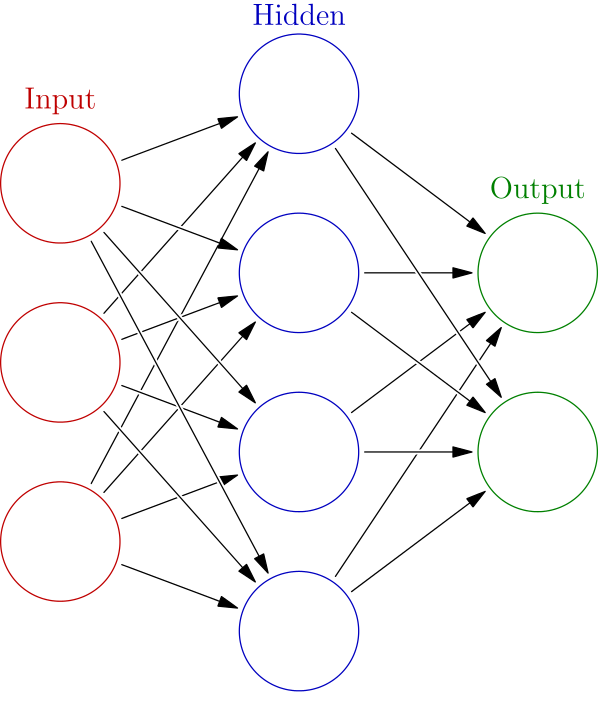
\includegraphics[width=.8\textwidth,height=.6\textwidth]{neuralNetwork}
\end{center}

As seen above neural networks have three main sections. The input, where information is input to the first layer. This information can range from pixel values of an image to stock price information over time. The Hidden, these layer(s) are used to develop relations between the input data. This is largely where the learning happens. The output, this last layer is where answers are given. This can come in many forms, from an array representing the percentage an answer is an image category to a single output that may represent the price of a stock. This architecture was developed with inspiration from the structure of neurons in the brain, hence the name. Just like the brain this structure can generalize problems very well and has extensive use in machine learning applications.\par

\subsubsection{Vanilla Network Experiment}
We ran an experiment during the UCF hackathon in order to see if a vanilla(network described above) could detect the differences within different types of insects. We sourced our data by scraping the website songofinsects.com. We were able to scrape just under one hundred sounds between three different species of insect; cicada, cricket, and katydid. Using these base files we then proceeded to split them into 5 second sections. This led us with over 200 sound files to sample from. For large networks this can be considered a very small amount of data. For future groups a much larger set of sounds should be used. These can be sourced from several Kaggle competitions.

\begin{center}
	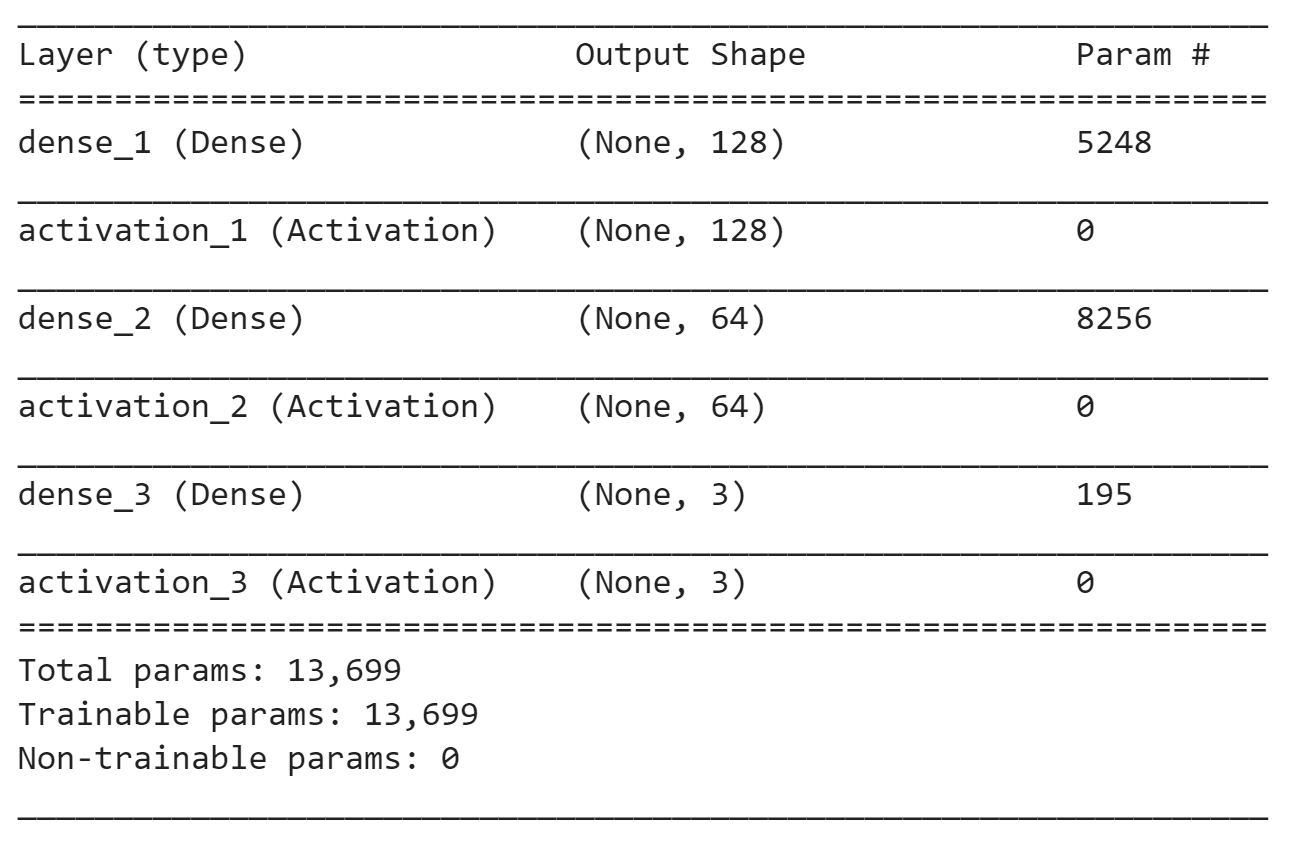
\includegraphics[width=.8\textwidth]{summary}
\end{center}

Using mfcc, a log scale frequency transformation, we pulled rough features out of the sound file and then fed them into our network. The structure of which can be seen above. With this set-up we were able to, on average, obtain a 53\% test accuracy, which is 20\% better than a random guess. Not spectacular results but promising results considering the lack of data and the small amount of layers in our network. Considerations for future groups could be larger data collection efforts along with securing hardware that can handle deeper networks. Code can be found in citation.\cite{ot}

\subsubsection{Convolution Neural Networks}
After this experiment we realized that vanilla networks would not be strong enough models to classify the sounds we needed. This led us to further research Convolution Neural Network. These models gain their name from the use of convolutions or kernels to find relations between data points. In our use these convolutions would be run across an image of a spectrograph made from a sound file. These convolutions would then be able to find low level features within the spectrograph that may detect certain types of sounds and be able to classify them. The only downside to this method is that it requires much more data than a vanilla network. We made some strides in collecting data for this process but were not able to make models in time for the end of the project. The data can be found at the citation.\cite{soundData}

\begin{figure}
	\centering
	\begin{minipage}{.5\textwidth}
		\centering
		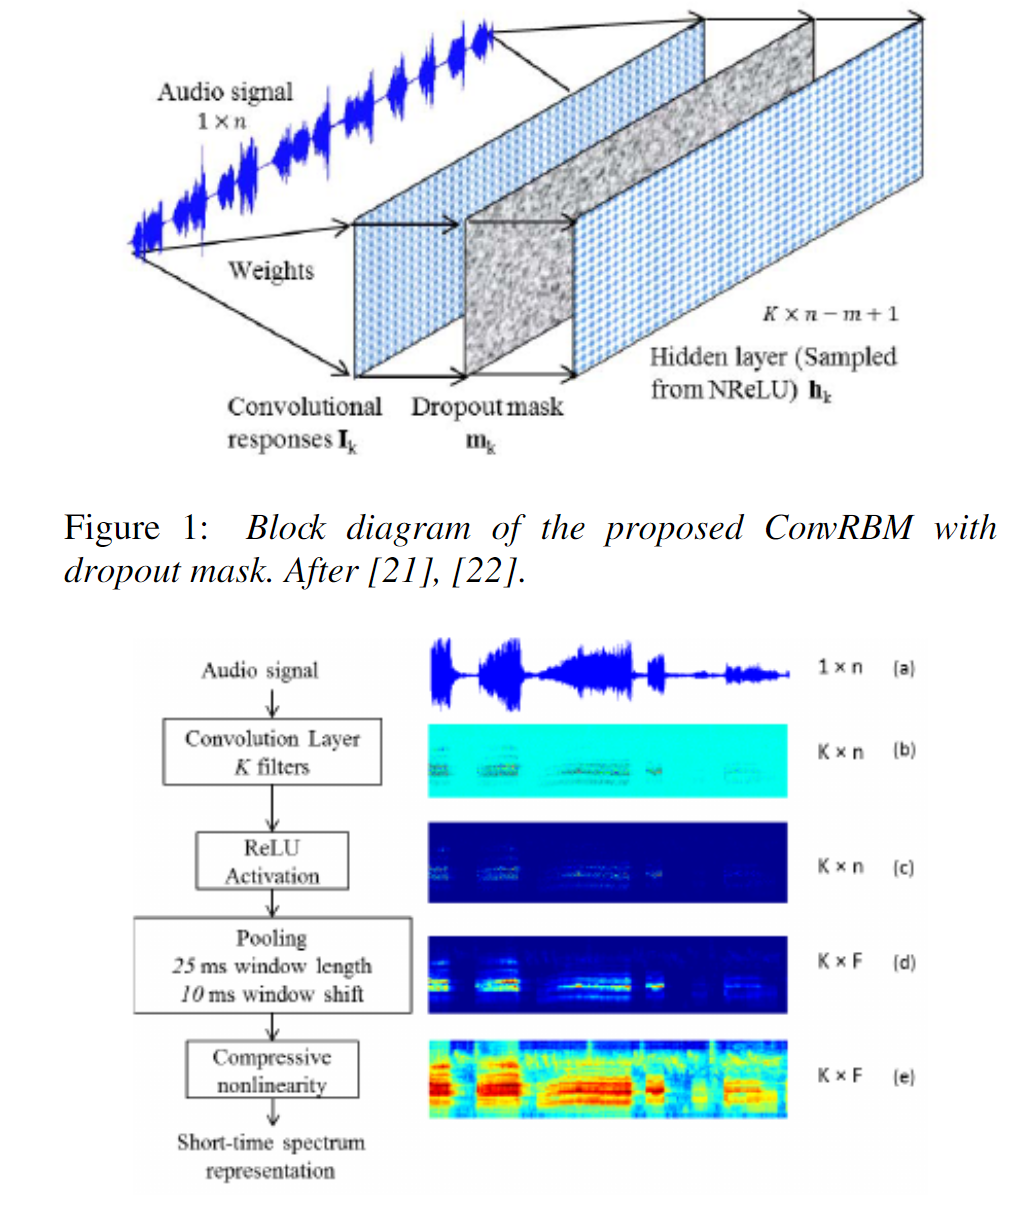
\includegraphics[width=.95\linewidth]{boltzmann}
		\captionof{figure}{ConvRBM}
		\label{fig:test1}
	\end{minipage}%
	\begin{minipage}{.5\textwidth}
		\centering
		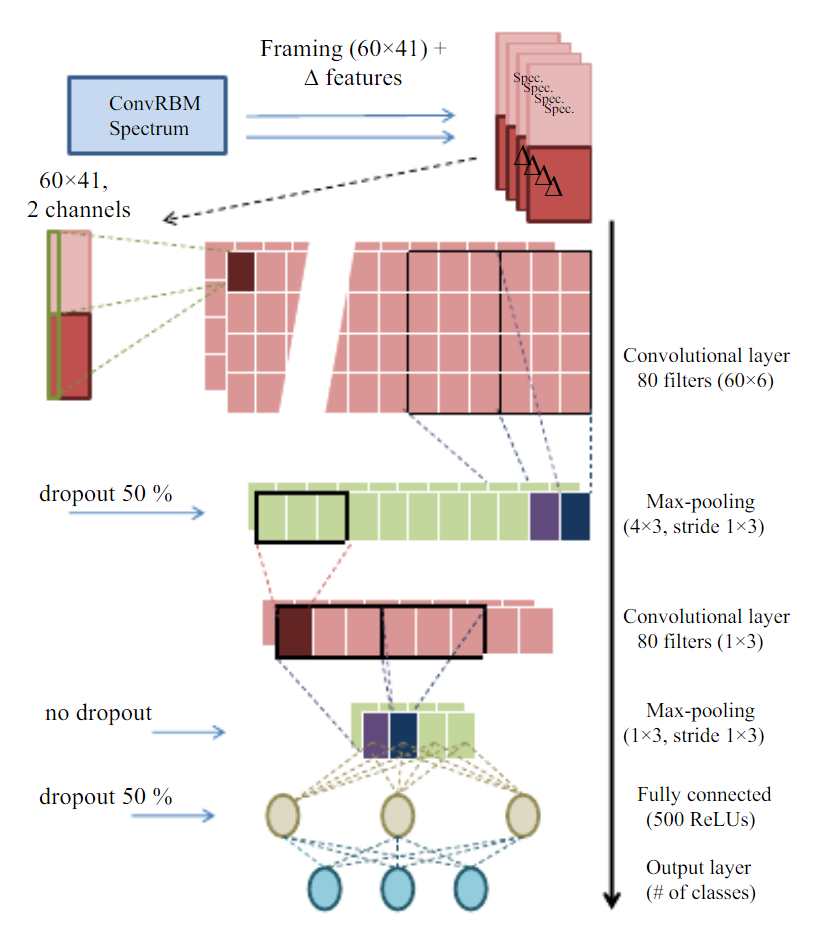
\includegraphics[width=.95\linewidth]{CNNClassifier}
		\captionof{figure}{ConvRBM/ CNN Classifier}
		\label{fig:test2}
	\end{minipage}
\end{figure}

\subsubsection{Boltzmann Machines}
While spectrograms are an amazing tool to represent the intensity of sound waves over frequencies, they do very little for feature extraction. The problem with this is that it obfuscates the feature extraction behind a layer of manipulation from audio to visual (via the spectrogram). With the use of Convolutional Restricted Boltzmann Machines the spectrograms can be manipulated to filter out the noise and extract features. This allows an image that can be more easily processed by the CNN.

Once the Boltzmann machine Spectrogaphs are made then a CNN classifier can be run on the image in order to extract the classifications. This method has been used on the EC-50\cite{EC50} data set, achieving a 78.45\% accuracy on a 5 fold validation. For future groups the ConvRBM code can be found here.\cite{ConvRBM}